\documentclass[10pt, compress, aspectratio=169, xcolor=table]{beamer}

\usetheme[numbering=none, progressbar=none, titleformat=smallcaps, sectionpage=none]{metropolis}

\usepackage{sourcecodepro}
\usepackage{booktabs}
\usepackage{array}
\usepackage{listings}
\usepackage{graphicx}
\usepackage{import}
\usepackage[english]{babel}
\usepackage[scale=2]{ccicons}
\usepackage{url}
\usepackage{relsize}
\usepackage{wasysym}

\usepackage{pgfplots}
\usepgfplotslibrary{dateplot}

\definecolor{Base}{HTML}{191F26}
\definecolor{Accent}{HTML}{157FFF}

\setbeamercolor{alerted text}{fg=Accent}
\setbeamercolor{frametitle}{bg=Base}

\setsansfont[BoldFont={Source Sans Pro Semibold},
              Numbers={OldStyle}]{Source Sans Pro}

\lstset{ %
  backgroundcolor={},
  basicstyle=\ttfamily\footnotesize,
  breakatwhitespace=true,
  breaklines=true,
  captionpos=n,
  commentstyle=\color{orange},
  escapeinside={\%*}{*)},
  extendedchars=true,
  frame=n,
  keywordstyle=\color{Accent},
  language=C++,
  rulecolor=\color{black},
  showspaces=false,
  showstringspaces=false,
  showtabs=false,
  stepnumber=2,
  stringstyle=\color{gray},
  tabsize=2,
  keywords={thrust,plus,device_vector, copy,transform,begin,end, copyin,
  copyout, acc, \_\_global\_\_, void, int, float, main, threadIdx, blockIdx,
  blockDim, if, else, malloc, NULL, cudaMalloc, cudaMemcpy, cudaSuccess,
  cudaGetLastError, cudaDeviceSynchronize, cudaFree, cudaMemcpyDeviceToHost,
  cudaMemcpyHostToDevice, const, data, independent, kernels, loop,
  fprintf, stderr, cudaGetErrorString, EXIT_FAILURE, for, dim3},
  otherkeywords={::, \#pragma, \#include, <<<,>>>, \&, \*, +, -, /, [, ], >, <}
}

\renewcommand*{\UrlFont}{\ttfamily\smaller\relax}

\graphicspath{{../img/}}

\title{Autotuning for High Performance Computing}
\author{\footnotesize Pedro Bruel \\ {\scriptsize \emph{phrb@ime.usp.br}}}
\institute{
\includegraphics[height=2cm]{imelogo}\\[0.2cm] Instituto de Matemática e Estatística \\ Universidade de São Paulo}
\date{\scriptsize \today}

\begin{document}

\begin{frame}
    \frametitle{CHStone Results: Naive Weights}
    \alert{CycloneV} final relative values to \alert{default} and
    \alert{random} starts, mean of \alert{10 tuning runs}, \alert{1.5h each}:
    \alert{Bluer} is \alert{better}
    \begin{columns}[T,onlytextwidth]
        \column{0.5\textwidth}
        \begin{center}
            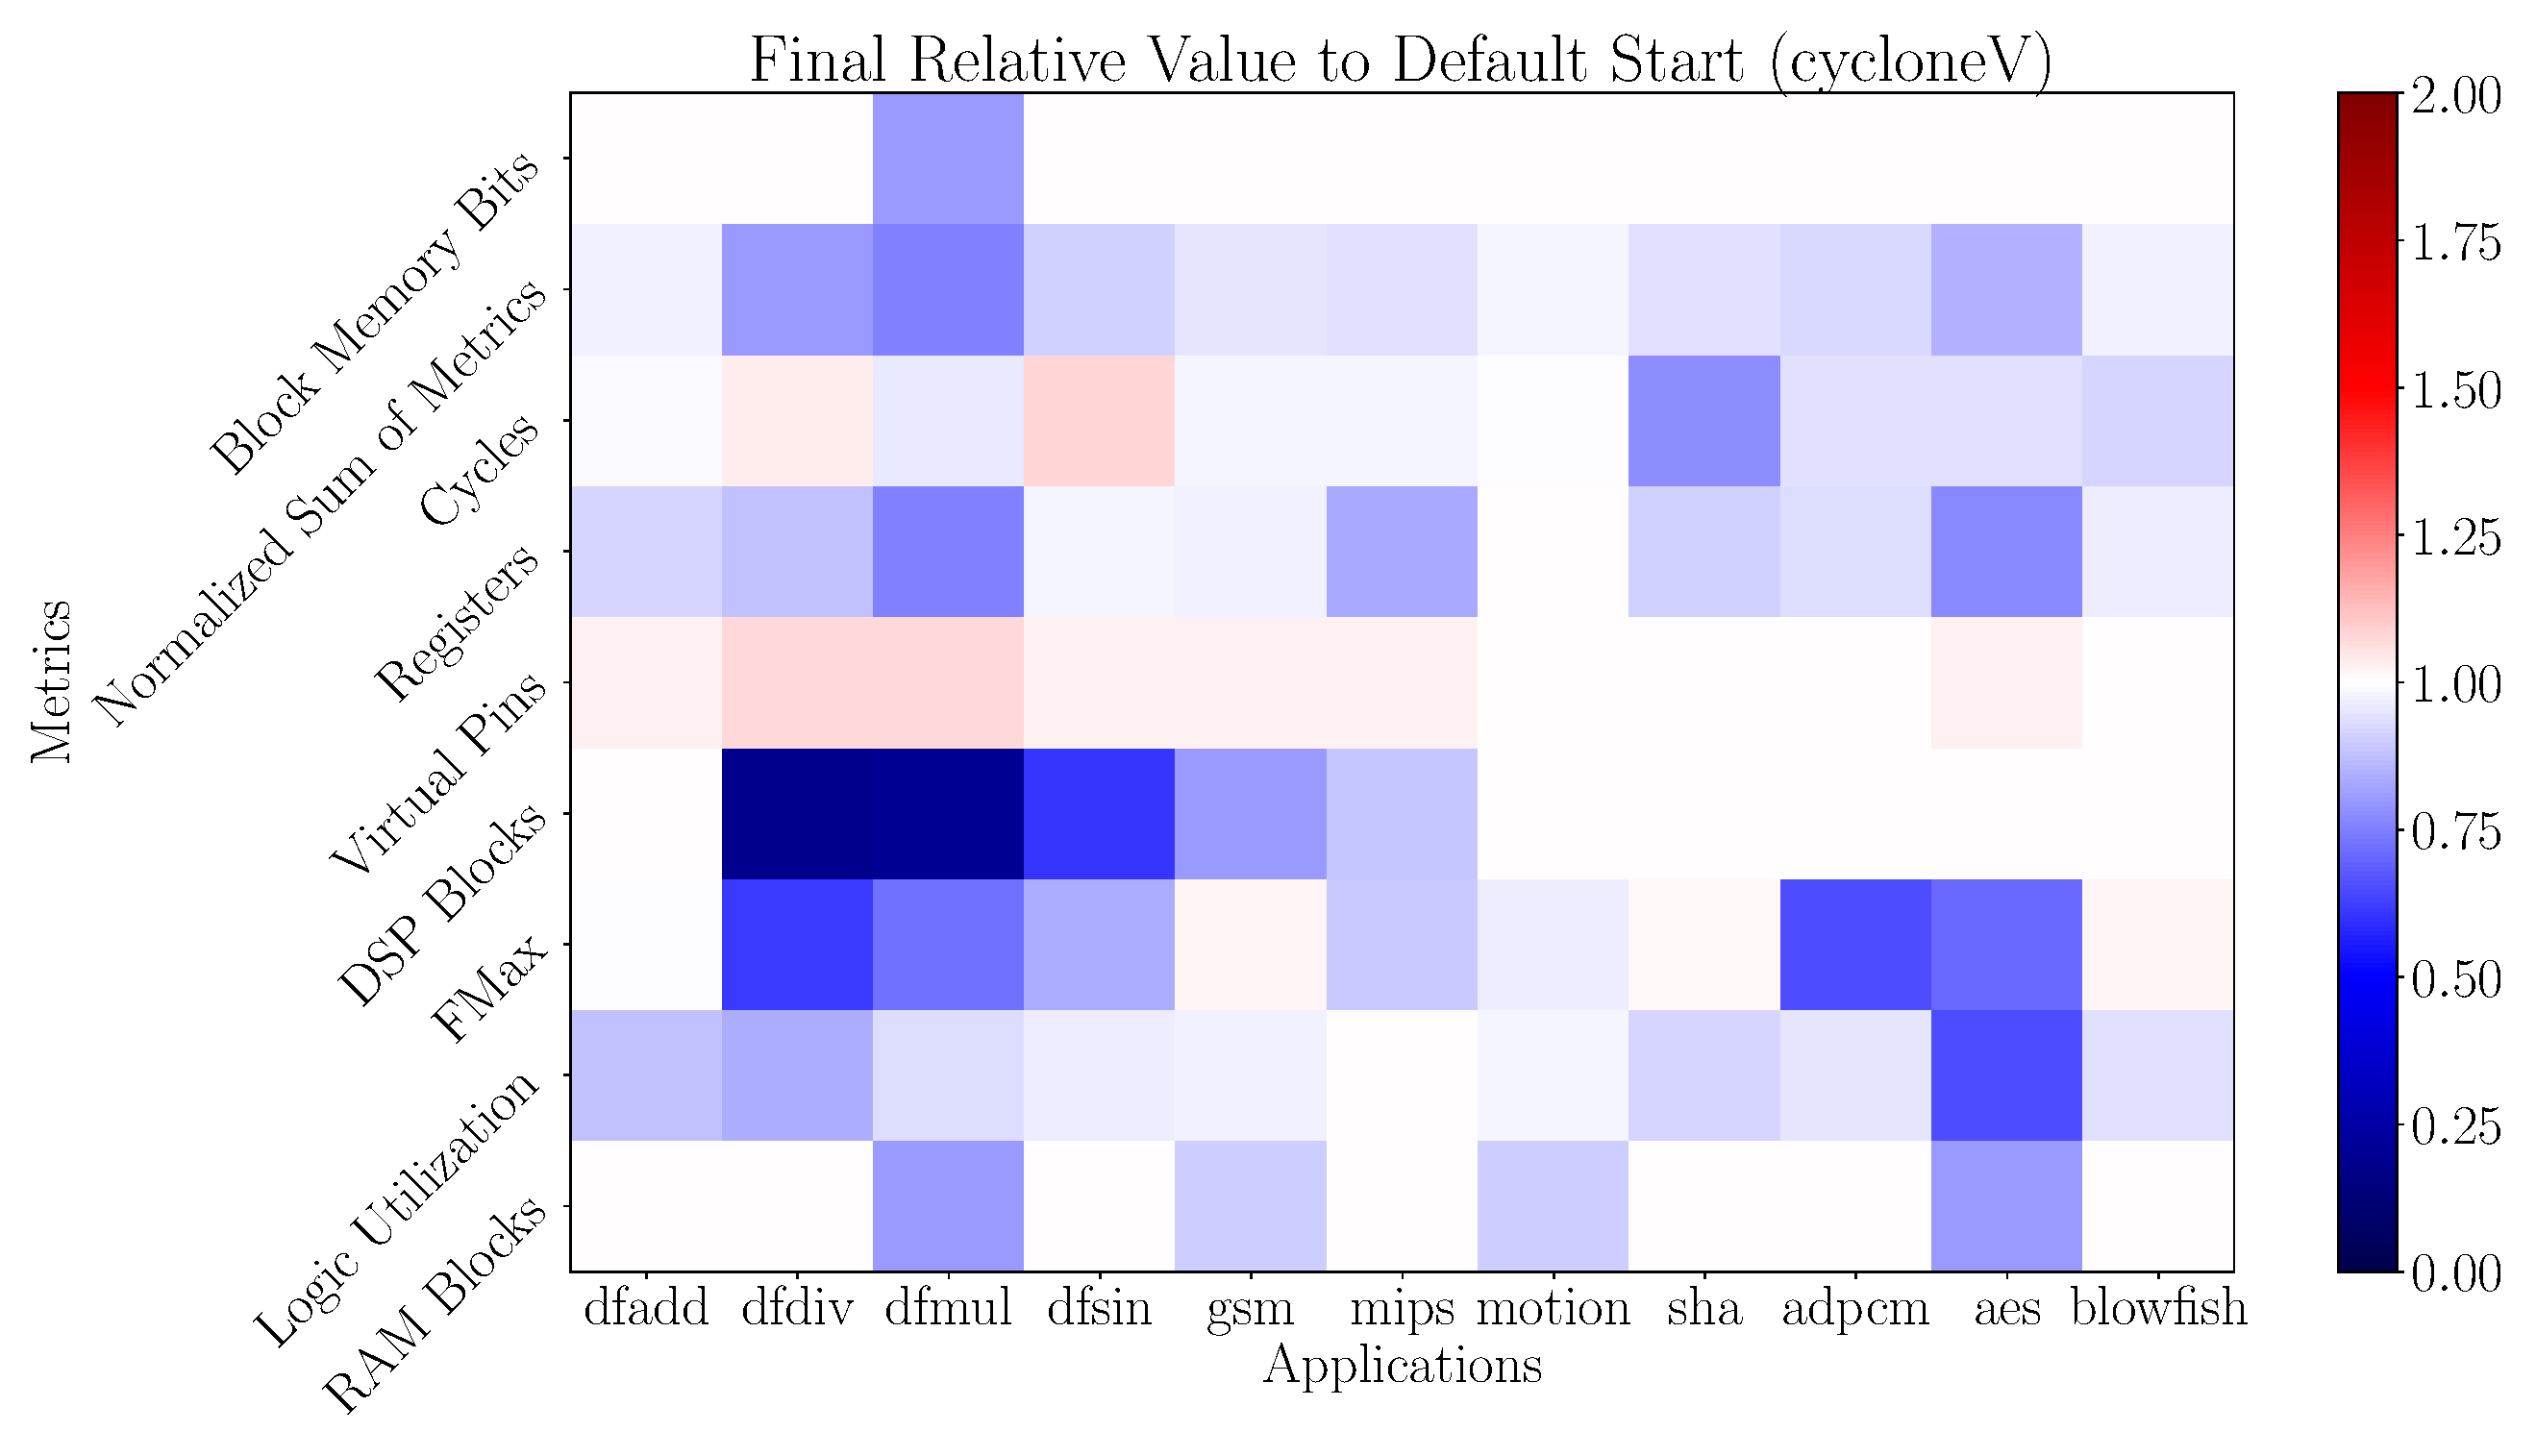
\includegraphics[width=\textwidth]{heatmap_default_cycloneV}
        \end{center}

        \column{0.5\textwidth}
        \begin{center}
            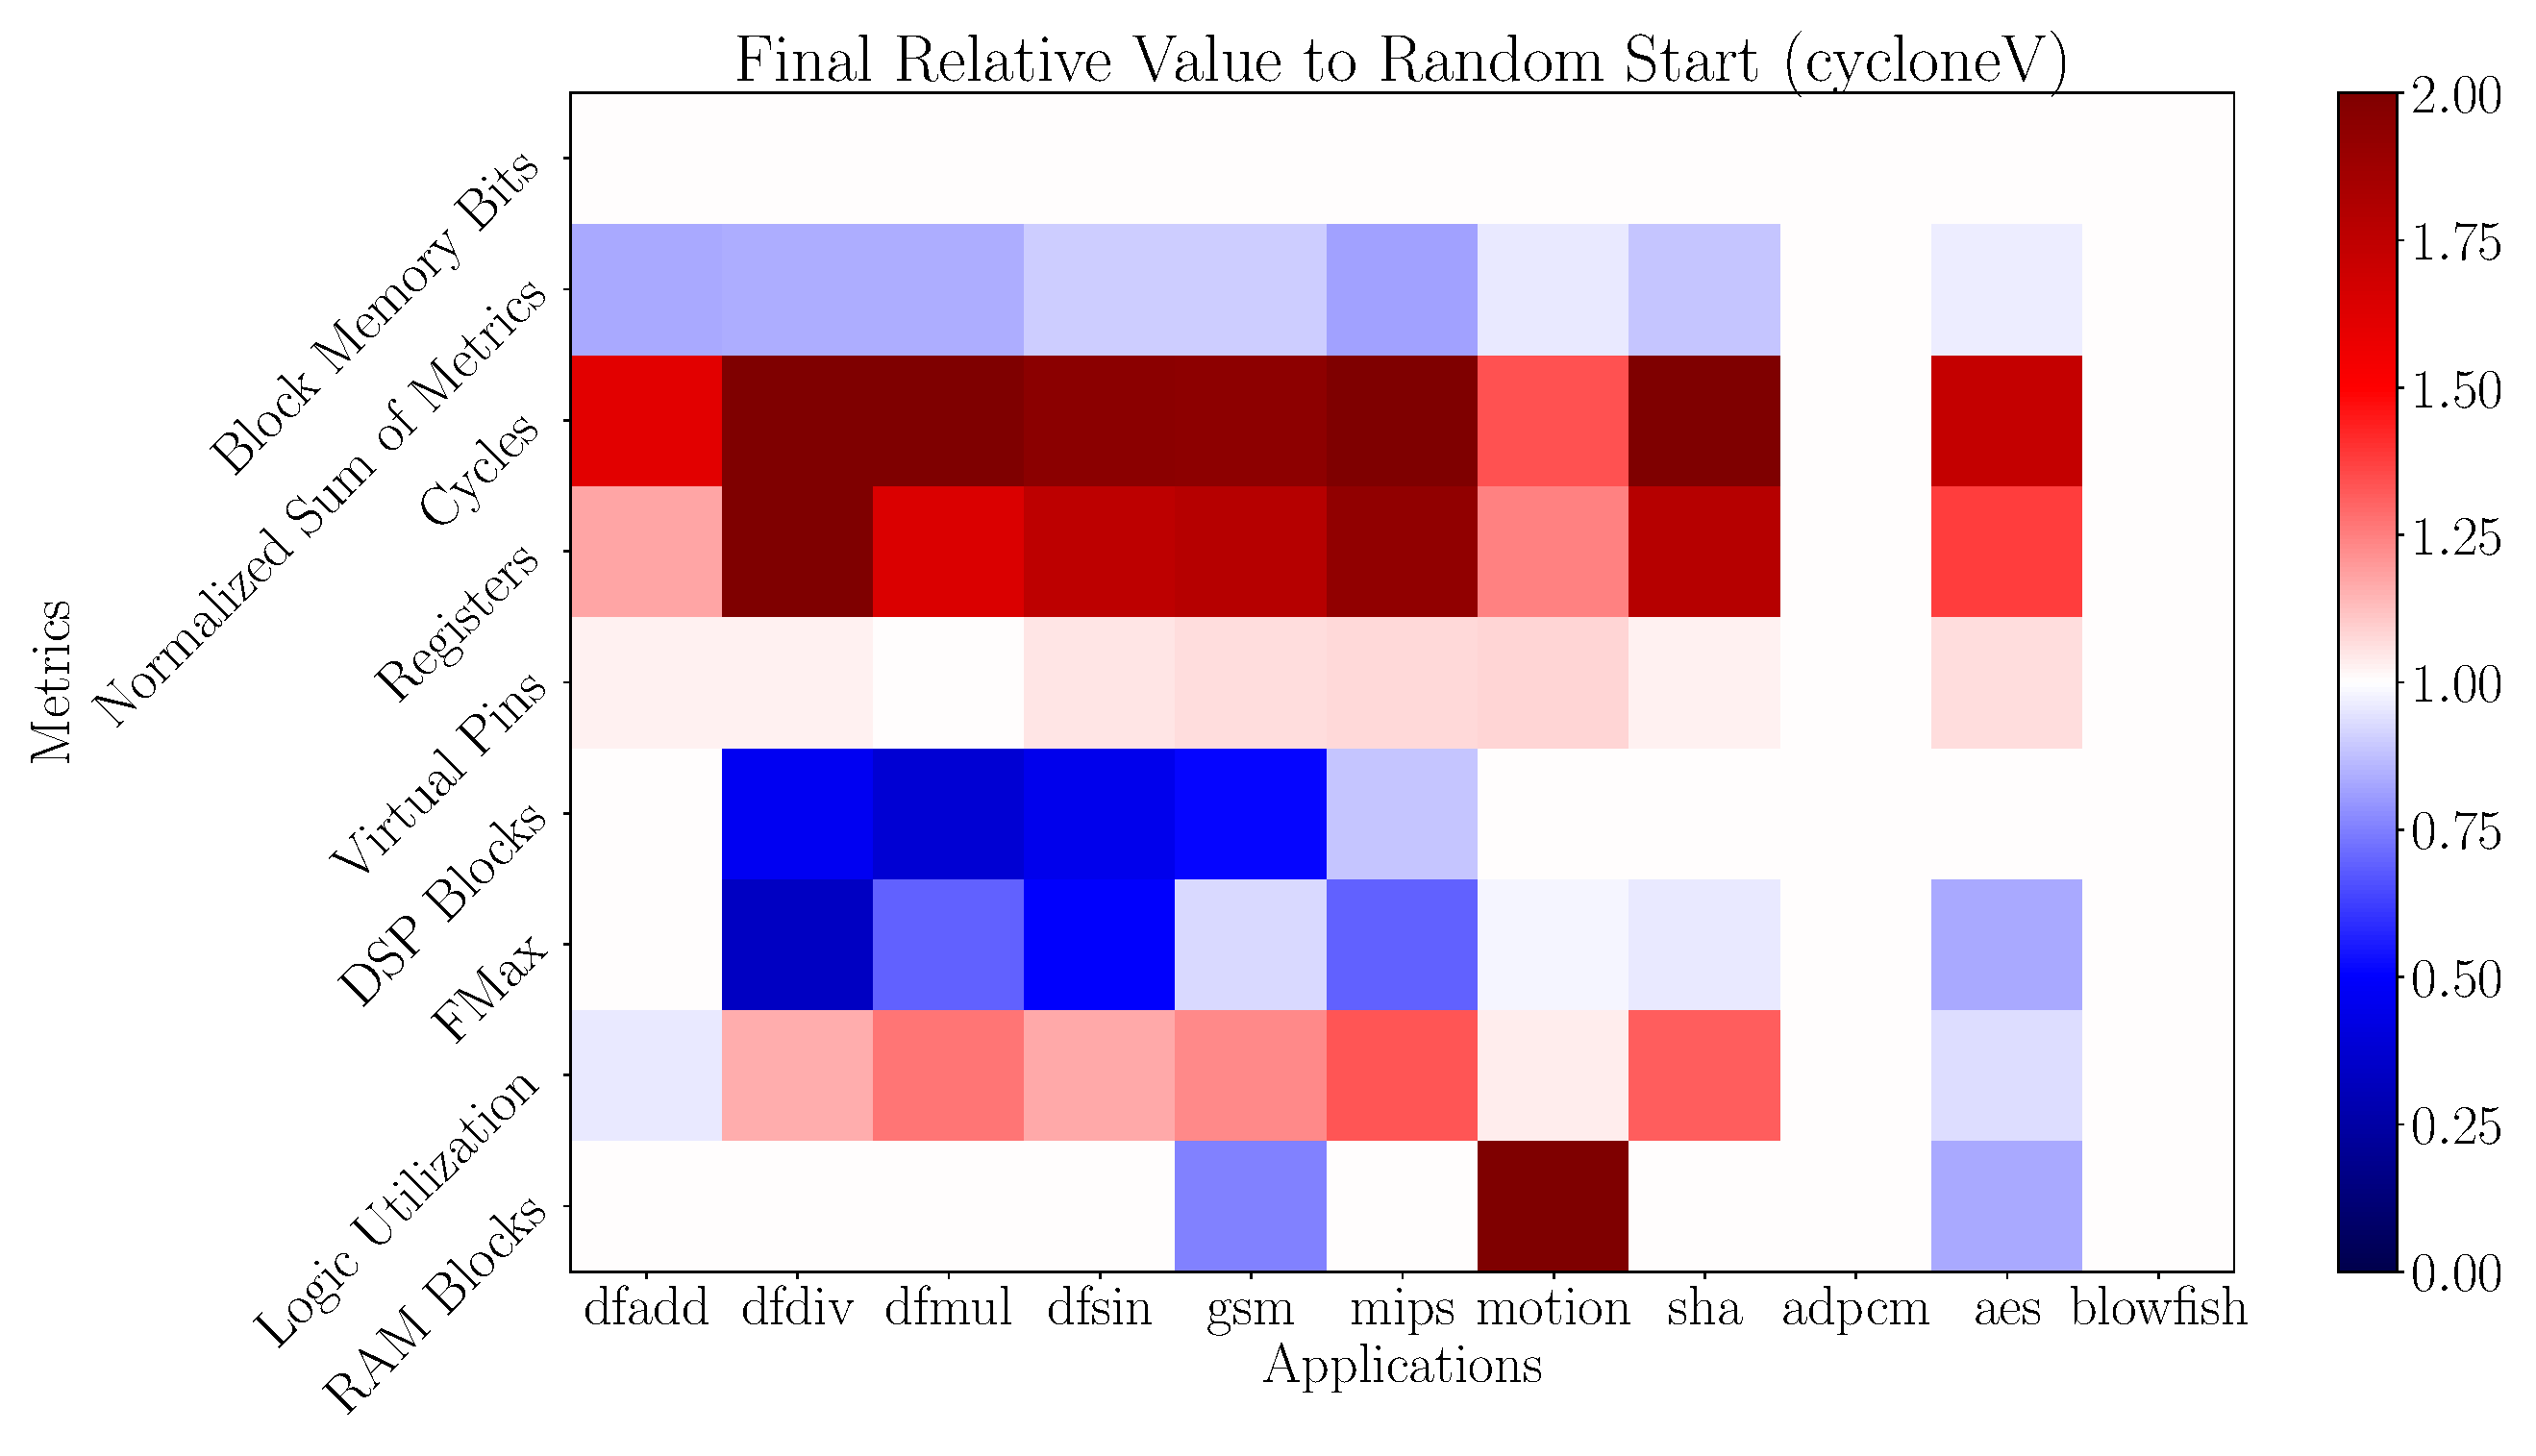
\includegraphics[width=\textwidth]{heatmap_random_cycloneV}
        \end{center}

    \end{columns}
\end{frame}

\begin{frame}
    \frametitle{CHStone Results: Naive Weights}
    \alert{StratixV} final relative values to \alert{default} and
    \alert{random} starts, mean of \alert{10 tuning runs}, \alert{1.5h each}:
    \alert{Bluer} is \alert{better}

    \begin{columns}[T,onlytextwidth]
        \column{0.5\textwidth}
        \begin{center}
            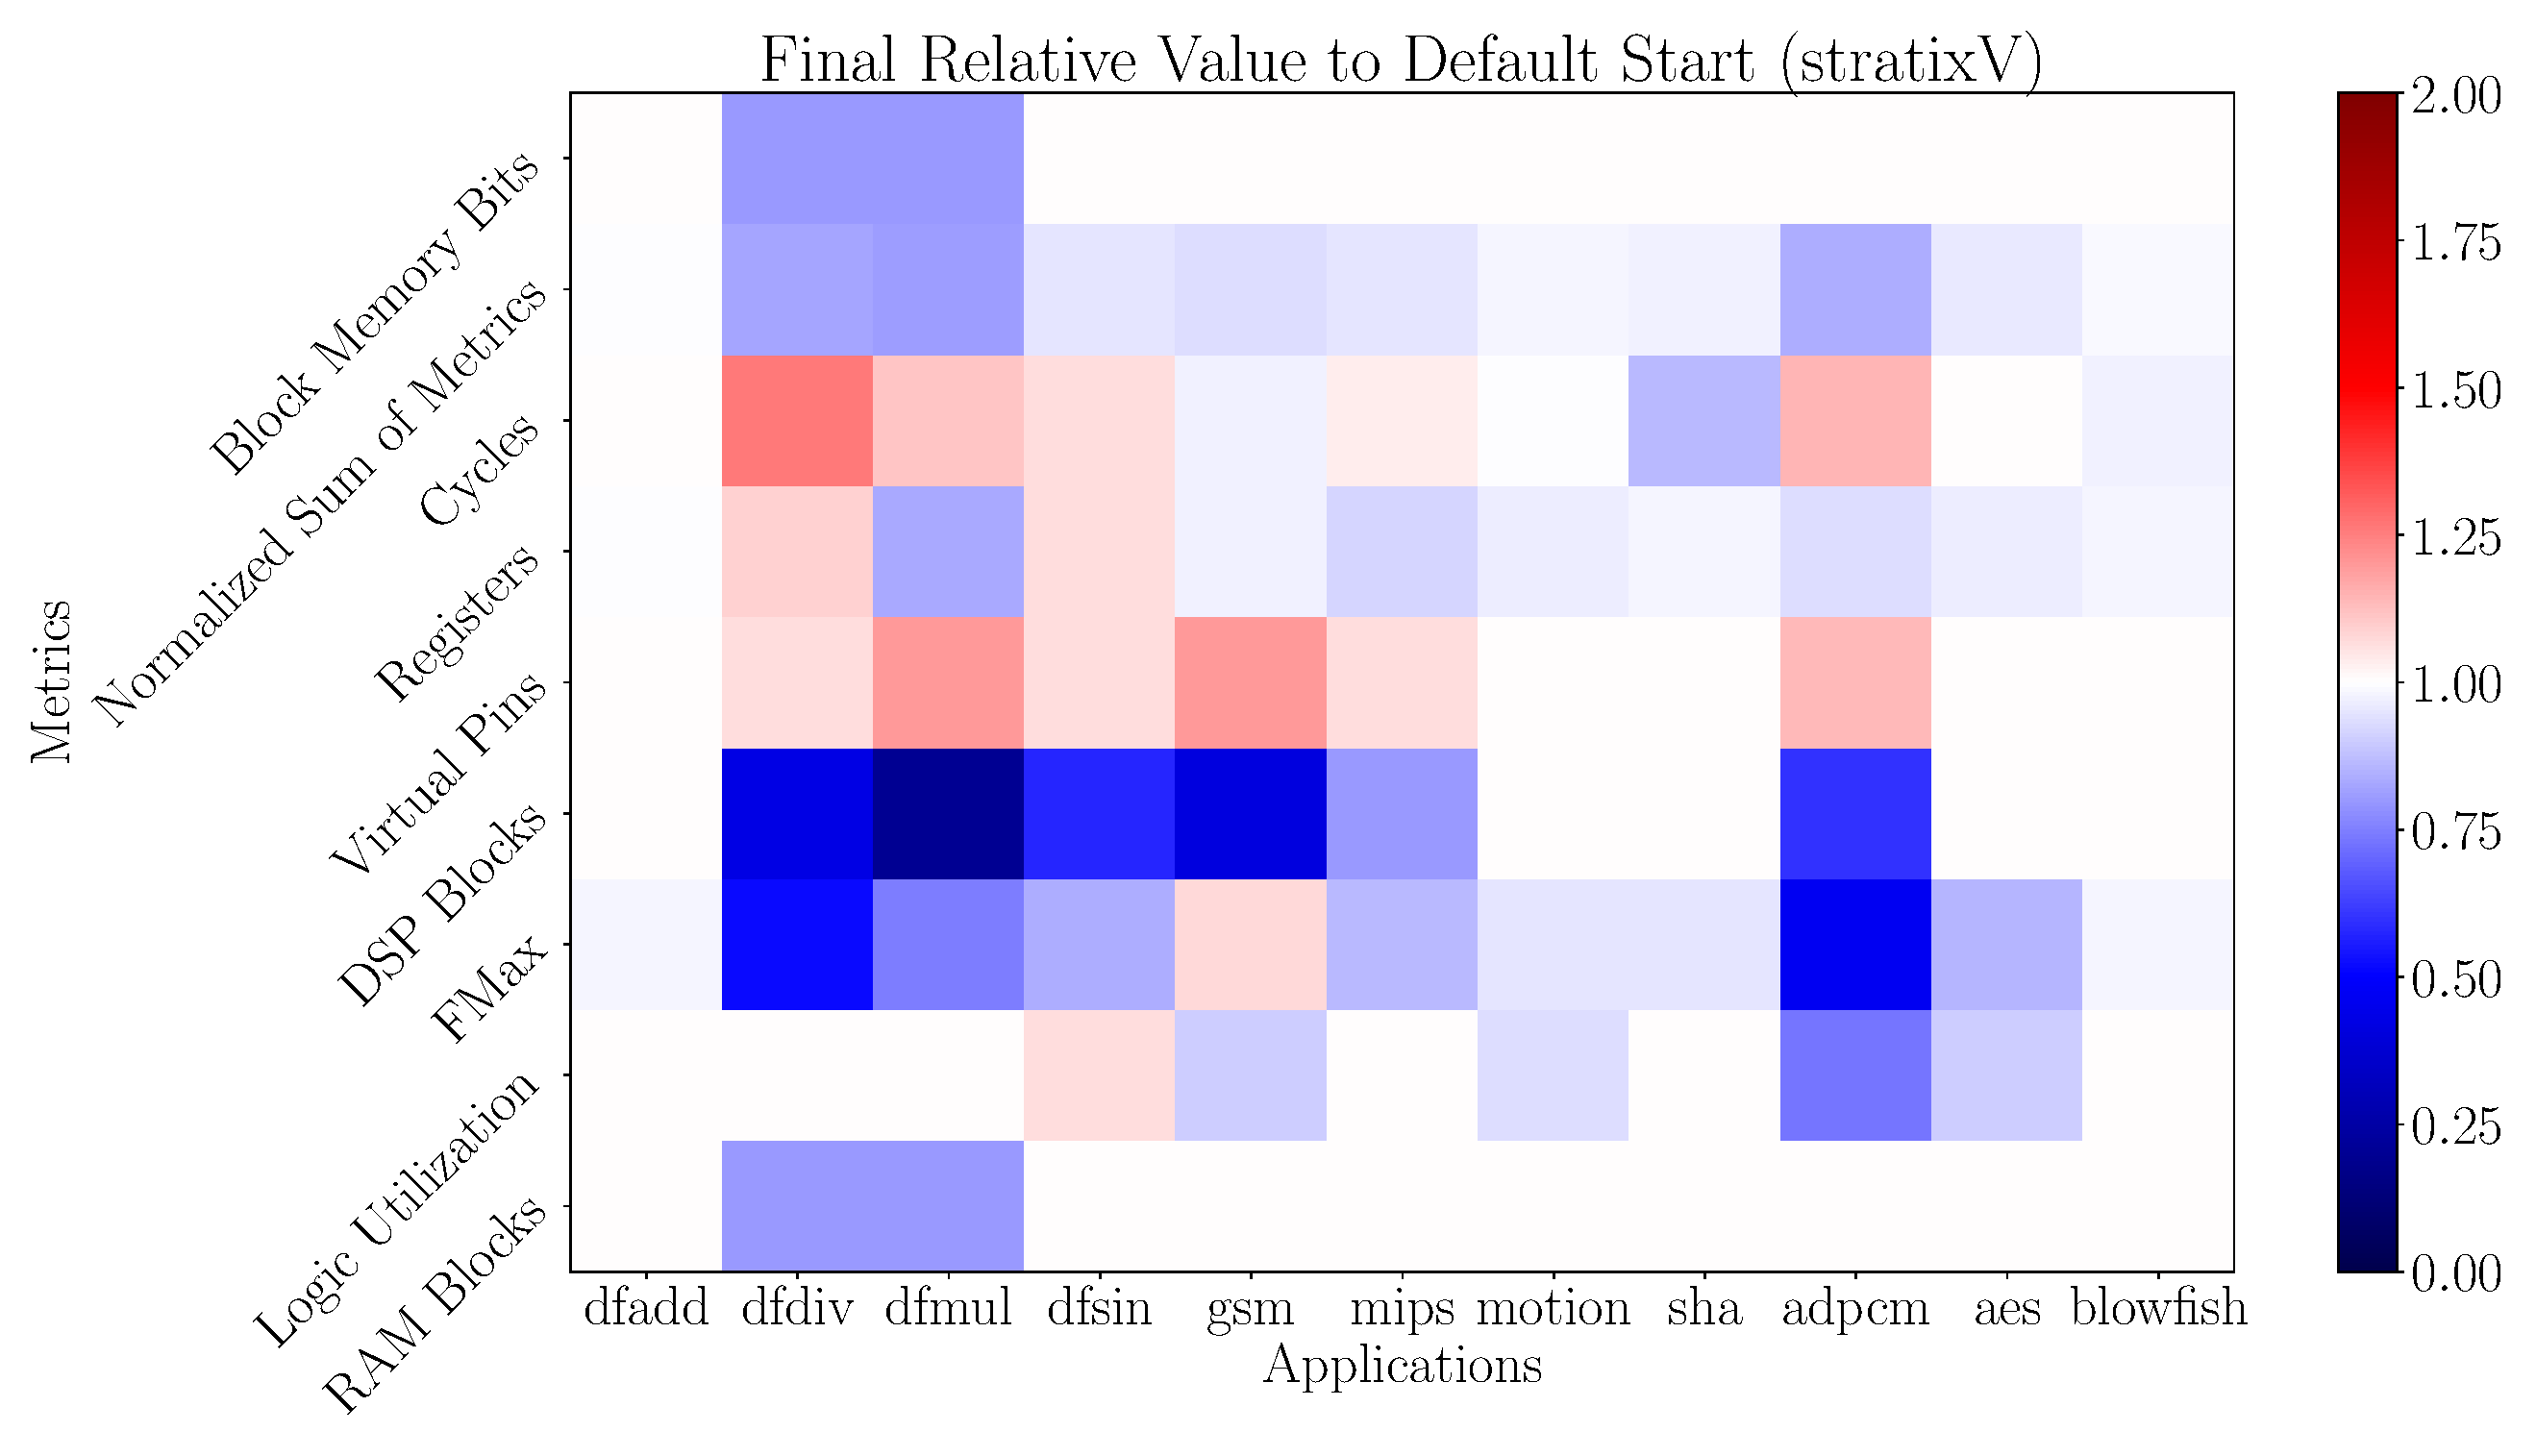
\includegraphics[width=\textwidth]{heatmap_default_stratixV}
        \end{center}

        \column{0.5\textwidth}
        \begin{center}
            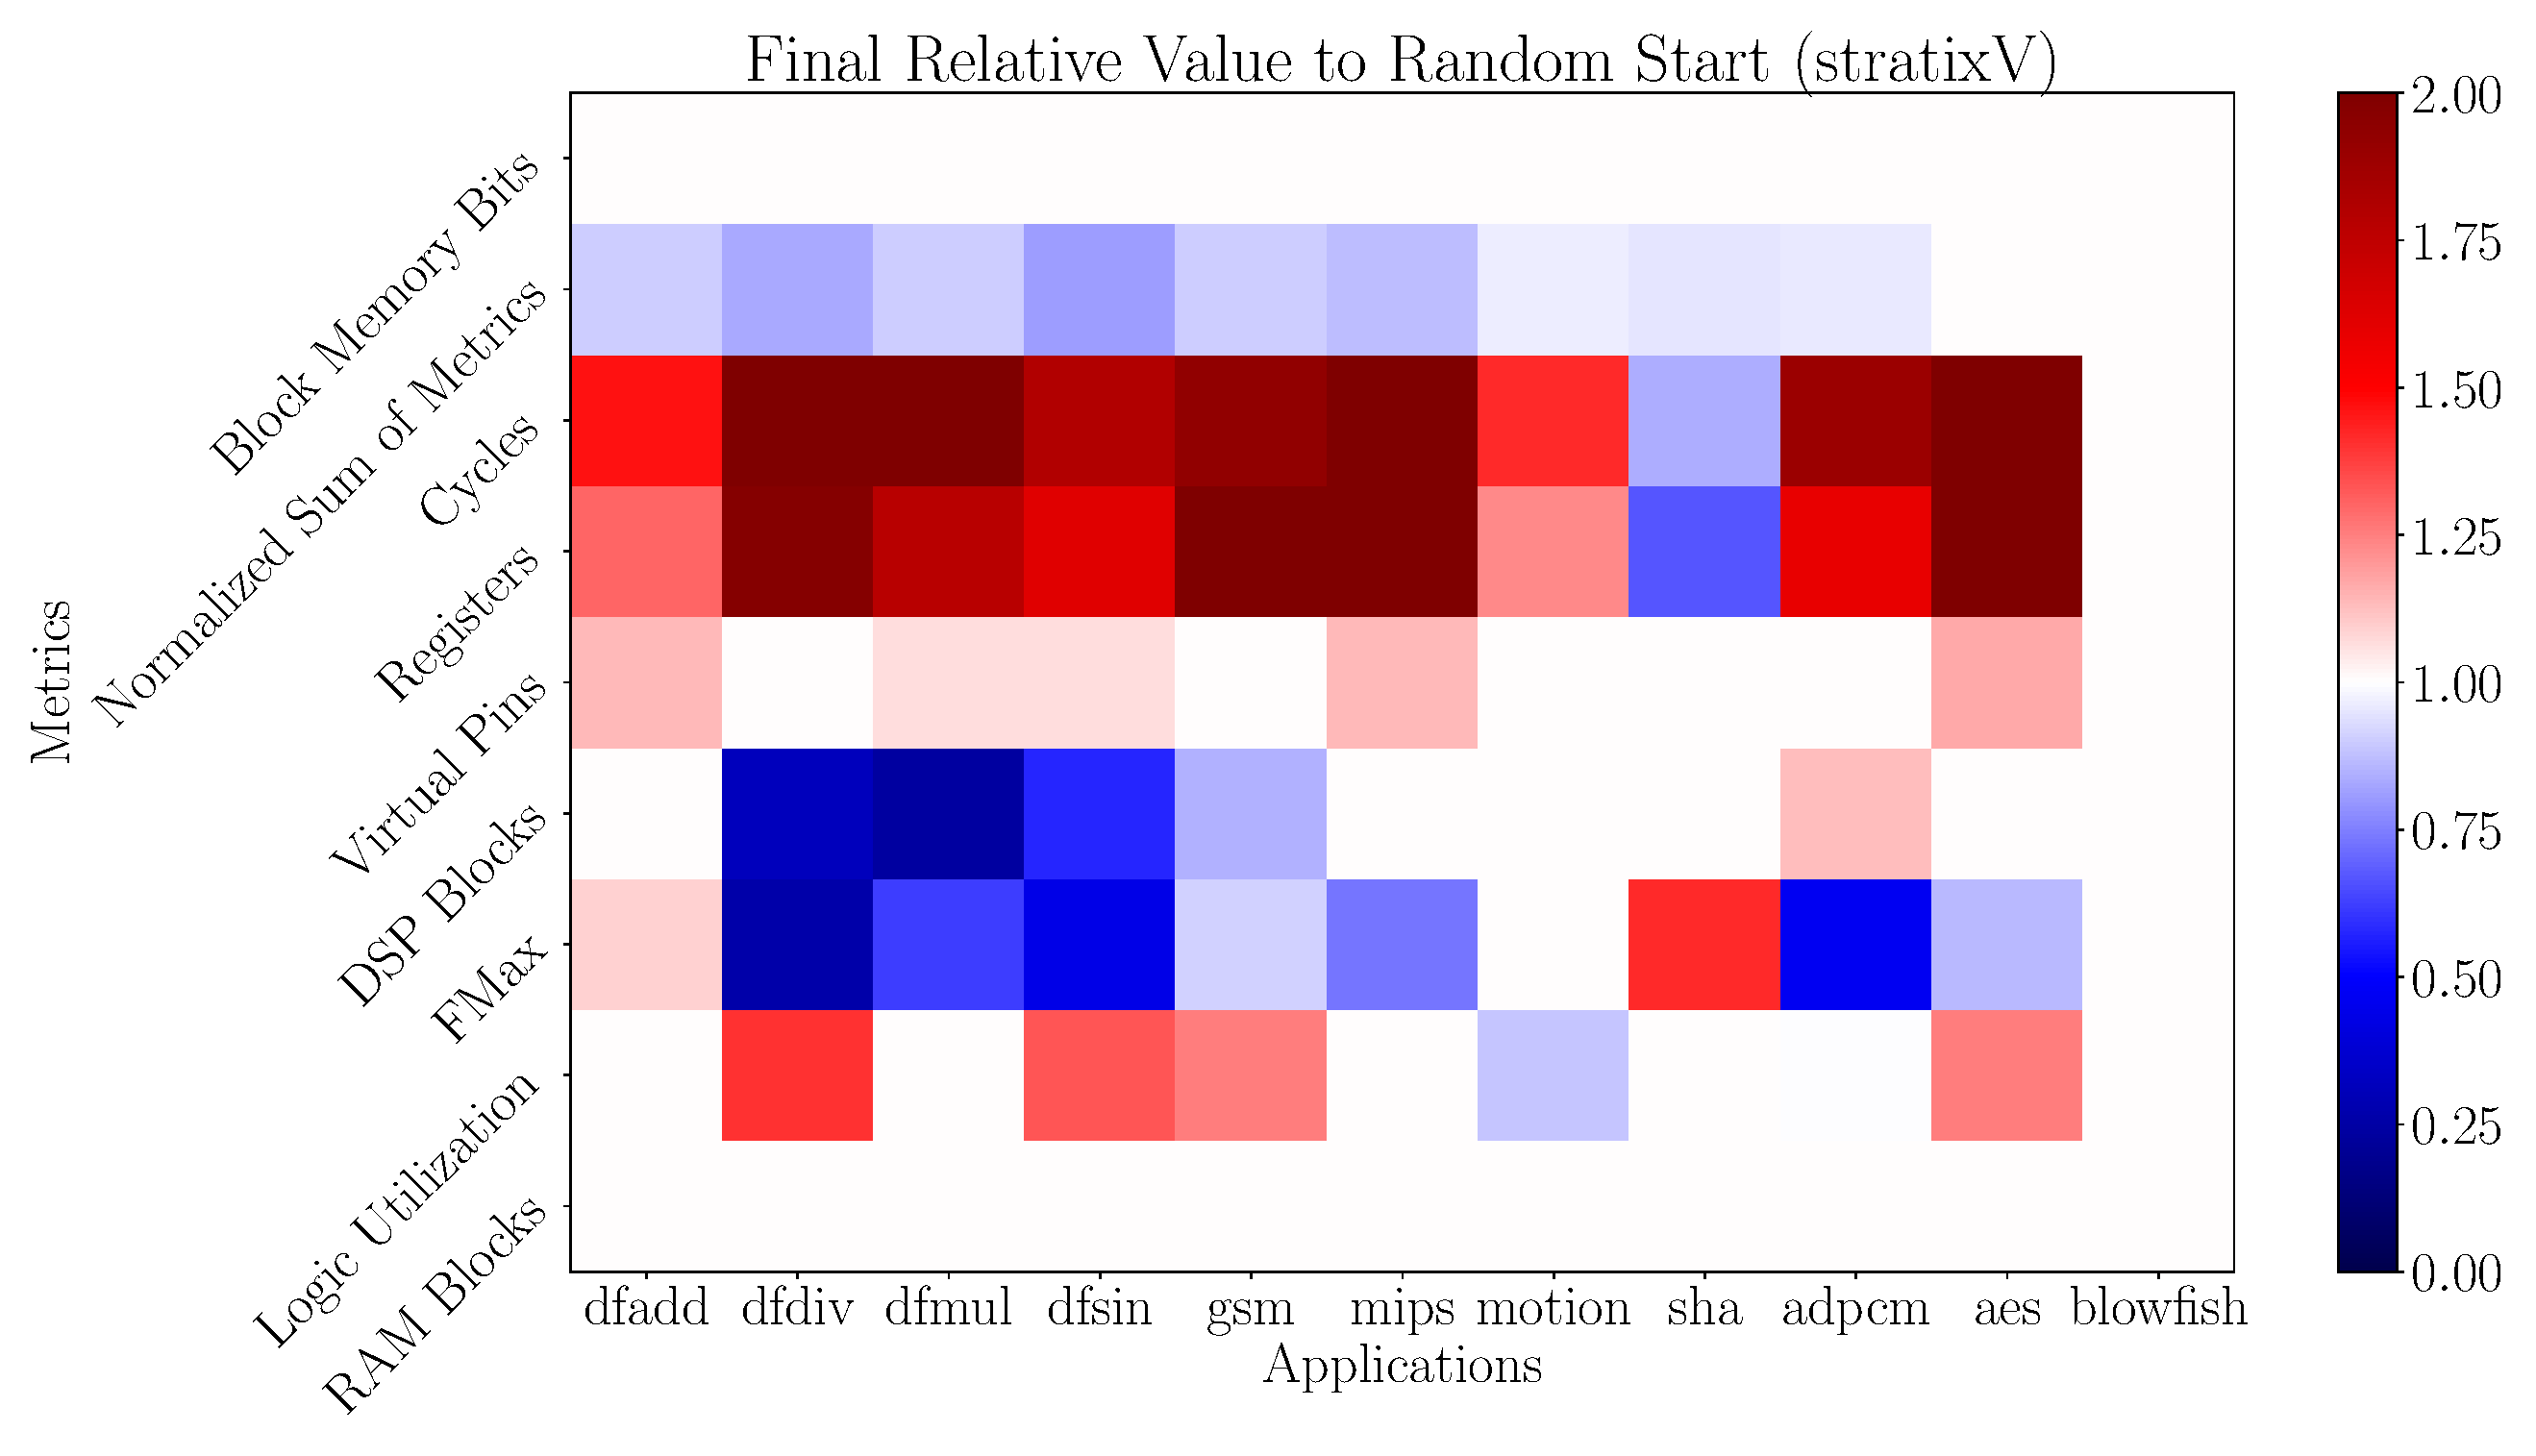
\includegraphics[width=\textwidth]{heatmap_random_stratixV}
        \end{center}

    \end{columns}
\end{frame}

\begin{frame}
    \frametitle{Contributions}
    \alert{Autotuning methodology}:
    \begin{itemize}
        \item Improve CHStone applications: \alert{meaningful} for HLS
        \item Combine \alert{multiple metrics in a simple way} provides good
            results
        \item \alert{Random vs. default} starts for autotuning HLS
        \item \alert{Meaningful set of metric weights}: is it possible to
            regain access to HPE machines?
    \end{itemize}
\end{frame}

\begin{frame}
    \frametitle{Autotuning LegUp Parameters for CHStone}
    Calculating the \alert{fitness function}:

    \begin{itemize}
        \item $M$: the set of \alert{metrics}
        \item $W$: the set of \alert{weights for each metric}
        \item $m_{i}^{0}$: \alert{initial measured value} for each metric
        \item $f(M,W)$: \alert{cost} or \alert{fitness function}, defined as
    \end{itemize}
    \begin{align*}
        f(M, W) = \dfrac{\sum\limits_{\substack{m_i \in M \\ w_i \in W}}{w_i\Big(\dfrac{m_i}{m_{i}^{0}}\Big)}}{\sum\limits_{w_i \in W}{w_i}}
    \end{align*}
    \begin{itemize}
        \item \alert{Naive weights}: $w_i = 1, \; \forall w_i \in W$
    \end{itemize}
\end{frame}

\begin{frame}[fragile]
    \frametitle{Meaningful Metric Weights}

    Relative weights in the \alert{scenarios devised by Sai}:

    \begin{table}[]
        \centering
        \begin{tabular}{@{}lcccccc@{}}
            \toprule
            Scenario & LUT & Registers & BRAMs & DSPs & FMax & Cyles \\ \midrule
            Area Efficient & \cellcolor[HTML]{32CB00} High & \cellcolor[HTML]{32CB00} High & \cellcolor[HTML]{32CB00} High & \cellcolor[HTML]{32CB00} High & \cellcolor[HTML]{FD6864} Low & \cellcolor[HTML]{FD6864} Low \\
            Performance + Latency & \cellcolor[HTML]{FD6864} Low & \cellcolor[HTML]{32CB00} High & \cellcolor[HTML]{FD6864} Low & \cellcolor[HTML]{FD6864} Low & \cellcolor[HTML]{32CB00} High & \cellcolor[HTML]{32CB00} High \\
            Performance & \cellcolor[HTML]{FD6864} Low & \cellcolor[HTML]{FFCC67} Medium & \cellcolor[HTML]{FD6864} Low & \cellcolor[HTML]{FD6864} Low & \cellcolor[HTML]{32CB00} High & \cellcolor[HTML]{FD6864} Low \\
            Balanced & \cellcolor[HTML]{FFCC67} Medium & \cellcolor[HTML]{FFCC67} Medium & \cellcolor[HTML]{FFCC67} Medium & \cellcolor[HTML]{FFCC67} Medium & \cellcolor[HTML]{FFCC67} Medium & \cellcolor[HTML]{FFCC67} Medium \\ \bottomrule
        \end{tabular}
    \end{table}
\end{frame}

\begin{frame}
    \frametitle{High-Level Synthesis for FPGAs: From C to Hardware}
    \begin{center}
        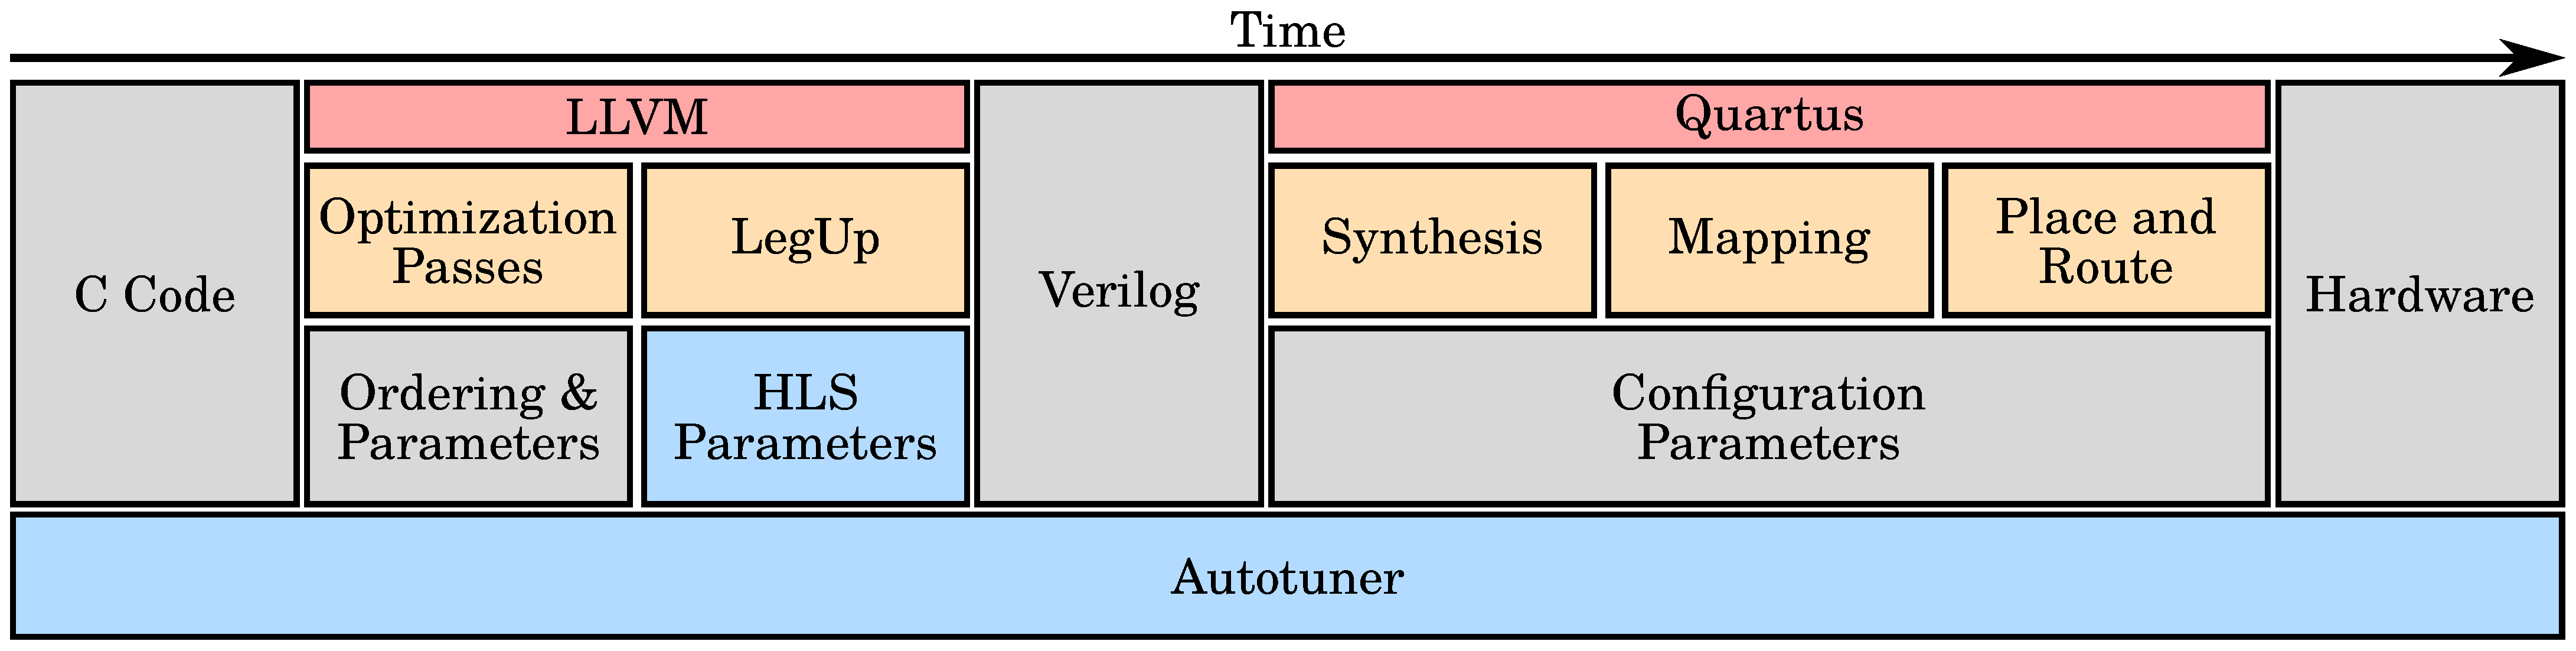
\includegraphics[width=1\textwidth]{fpga-stack}
    \end{center}

    \begin{itemize}
        \item We tuned applications from the \alert{CHStone Benchmark Suite}
        \item C $\rightarrow$ Verilog: takes \alert{seconds}; \alert{\textasciitilde16\% speedup}
        \item Verilog $\rightarrow$ Hardware: takes \alert{minutes}, \alert{hours}; \alert{10\%-2x speedup}
        \item We tuned C $\rightarrow$ Verilog, but had \alert{to pay the cost} of Verilog $\rightarrow$ Hardware
    \end{itemize}
\end{frame}

\end{document}
